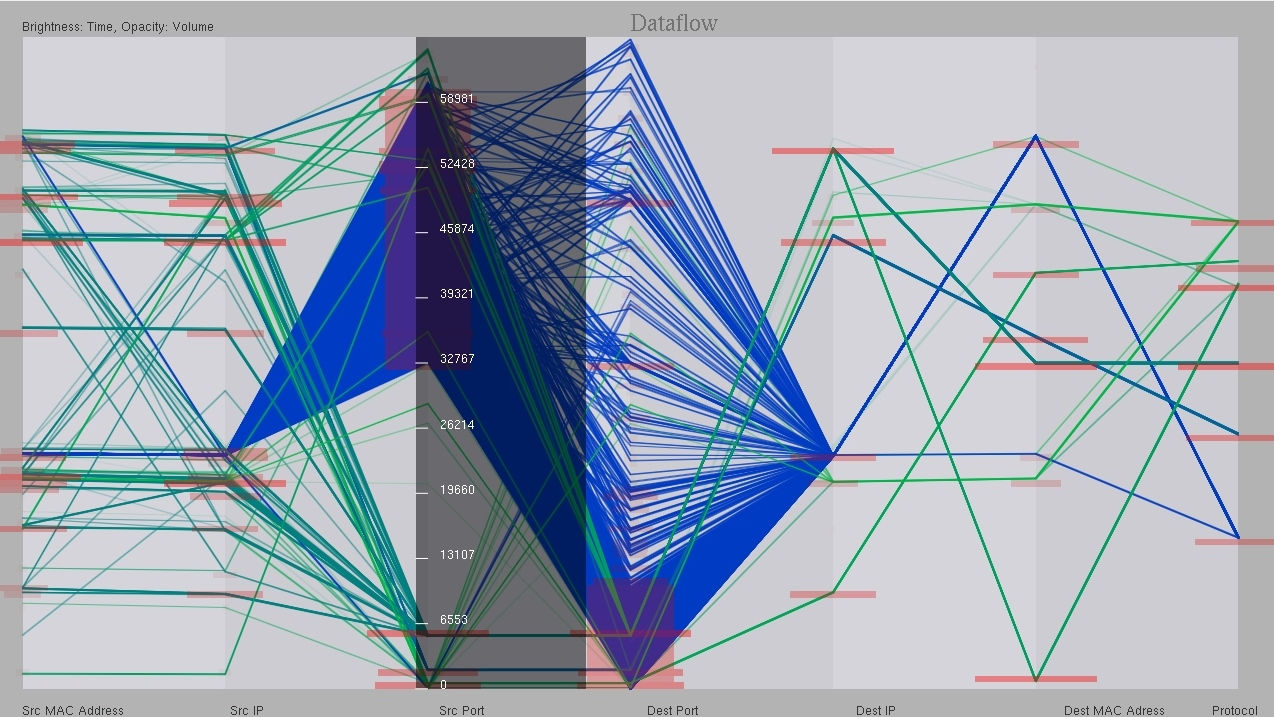
\includegraphics[width=\linewidth]{materials/dataflow.jpg}
The Data Flow visualization applies the idea of parallel coordinates proposed by \cite{inselberg1985plane} to network traffic. Following the principles layed out in \cite{fliggnetwork} the visualization shows the `flow' of each packet, representing each as a line through the parallel coordinates. This provides an informative view of the whole traffic in the network. It visualises the distribution of various packet attributes while also giving an intuitive insight into relationships and correlations between distinct aspects of the packets.

Lines representing packets are coloured based on their value in some coordinate. They fade out based on how old the packet is, thereby placing focus on newer developments in the network. 

A common criticism of parallel coordinate plots is that they make it hard to interpret data that is uniformly distributed between coordinates or that is very concentrated around few values \cite{marty2009applied}. Our implementation addresses these concerns using animation. Lines representing new packets are randomly perturbed and move slightly. This makes it easier to spot whether a line represents one or more packets. The animation allows the user to distinguish between single packets and concentrated groups of packets with the same characteristics.

Suppose, for example, that multiple requests to a server come from a single MAC address through the same ports and using the same protocol. A non-animated visualization would represent all these requests as a single line. A user would erroneously interpret this as a single request. Adding randomness makes the pack of requests more visible without significantly impacting the accuracy of the data representation.

The Data FLow visualization is closely tied to the previously described Attribute Distribution visualization. If a coordinate shows an unusual distribution (say a uniform use of ports in a certain range), then a single click on the packets in this coordinate will show the Attribute Distribution log plot which allows direct access to filtering option. Hovering over packets also displays further contextual information.